\documentclass[sigplan,review,anonymous]{acmart}\settopmatter{printfolios=true,printccs=false,printacmref=false}

\usepackage{fancyvrb}
\usepackage{xcolor}
\usepackage{amssymb} 
\usepackage{tikz}
\usepackage[autostyle]{csquotes}
\usepackage{listings}
\usepackage{multirow}
\synctex=1
\usepackage{pgfplots}

\usetikzlibrary{positioning}
\usetikzlibrary{arrows,automata}
\sloppy


%%%%%%%%%%%%%%%%%%%%%%%%%%%%%%%%%%%%%%%%%%%%%%%%%%%%%%%%%%%%%%%%%%%%%%%%%%%%%%
\begin{document}
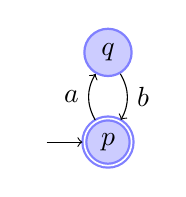
\begin{tikzpicture}
	\tikzset{state/.style={circle,draw=blue!50,fill=blue!20,
			thick,inner sep=0pt,minimum size=6mm}, initial text=$ $}

\node[state,initial,accepting] (q0) {$p$};

\node[state] (q01) [above = 0.5cm of q0] {$q$};

\draw[->] (q0) edge [bend left] node [left]{$a$} (q01) ;
\draw[->] (q01) edge [bend left] node [right]{$b$} (q0) ;
\end{tikzpicture}

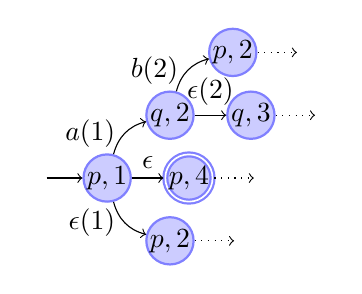
\begin{tikzpicture}
\tikzset{state/.style={circle,draw=blue!50,fill=blue!20,
		thick,inner sep=0pt,minimum size=6mm}, initial text=$ $}

\node[state,initial] (q0) {$p,1$};

\node[state] (q01) [above right = 0.5cm of q0] {$q,2$};

\node[state] (q02) [below right = 0.5cm of q0] {$p,2$};

\node[state,accepting] (q03) [ right = 0.4cm of q0] {$p,4$};

\node[state] (q11) [above right = 0.5cm of q01] {$p,2$};

\node[state] (q12) [ right = 0.4cm of q01] {$q,3$};

\node (q02d) [ right = 0.5cm of q02] {};
\draw[dotted,->] (q02) edge (q02d) ;

\node (q03d) [ right = 0.5cm of q03] {};
\draw[dotted,->] (q03) edge (q03d) ;

\node (q12d) [ right = 0.5cm of q12] {};
\draw[dotted,->] (q12) edge (q12d) ;

\node (q11d) [ right = 0.5cm of q11] {};
\draw[dotted,->] (q11) edge (q11d) ;

\draw[->] (q0) edge [bend left] node [left]{$a(1)$} (q01) ;
\draw[->] (q0) edge [bend right] node [left]{$\epsilon(1)$} (q02) ;
\draw[->] (q0) edge node [above]{$\epsilon$} (q03) ;

\draw[->] (q01) edge [bend left] node [left]{$b(2)$} (q11) ;
\draw[->] (q01) edge node [above]{$\epsilon(2)$} (q12) ;
\end{tikzpicture}

\end{document}
%%%%%%%%%%%%%%%%%%%%%%%%%%%%%%%%%%%%%%%%%%%%%%%%%%%%%%%%%%%%%%%%%%%%%%%%%%%%%%
